% Copyright 2023 Kieran W Harvie. All rights reserved.

\newcommand{\uline}[1]{|\text{#1}|}

\section{Causal Metric}
\subsection{Basic Geometry}
Consider two points A and B that we wish to find the area of the rectangle between them in terms of their coordinates on an axis at a $45^\circ$ angle.
\\

\begin{center}
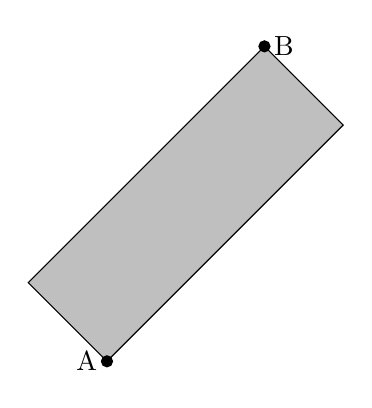
\begin{tikzpicture}
\fill [fill=lightgray] (0,0) -- (-1,1) -- (2,4) -- (3,3) -- cycle;
\draw  [latex-latex](0,0) -- (-1,1) -- (2,4)-- (3,3) -- cycle;

\filldraw (0,0) node[left] {A} circle (2pt);
\filldraw (2,4) node[right]{B} circle (2pt);
\end{tikzpicture}
\end{center}

Drop an altitude from B to line up horizontally with A and label the end-point D.
The length |AD| and |BD| are the coordinates.

\begin{center}
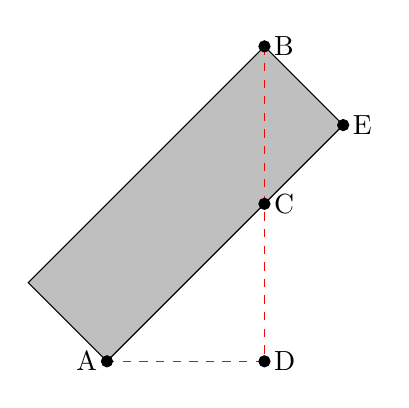
\begin{tikzpicture}
\fill [fill=lightgray] (0,0) -- (-1,1) -- (2,4) -- (3,3) -- cycle;
\draw  [latex-latex](0,0) -- (-1,1) -- (2,4)-- (3,3) -- cycle;

\draw[dashed,red] (2,4)-- (2,2)--(2,0) -- (0,0);

\filldraw (0,0) node[left] {A} circle (2pt);
\filldraw (2,4) node[right]{B} circle (2pt);
\filldraw (2,2) node[right]{C} circle (2pt);
\filldraw (2,0) node[right]{D} circle (2pt);
\filldraw (3,3) node[right]{E} circle (2pt);
\end{tikzpicture}
\end{center}

The triangles $\triangle$ACD and $\triangle$BCE are $45^\circ-90^\circ-45^\circ$ triangles meaning:
\begin{equation*}
\begin{aligned}
	\uline{AC} =& \sqrt{2}\uline{AD} \\
	\uline{BE} =& \frac{1}{\sqrt{2}}\uline{BC} \\
	=& \frac{1}{\sqrt{2}}(\uline{BD}-\uline{CD}) \\
	=& \frac{1}{\sqrt{2}}(\uline{BD}-\uline{AD}) \\
\end{aligned}
\end{equation*}

Hence the (signed) area of the rectangle is:
\begin{equation*}
\begin{aligned}
	\uline{BE}\cdot\uline{AE} =&\uline{BE}\cdot(\uline{AC}+\uline{CE}) \\
	=&(\uline{BD}-\uline{AD})(\uline{BD}+\uline{AD})\\
	=&\uline{BD}^2-\uline{AD}^2\\
\end{aligned}
\end{equation*}

\subsection{Causal Metric}
This construction supplies some intuition for Minkowski Metric.
Since if we interpret the plane as the set of events where the horizontal component is space-like and the vertical is time-like.
The reason the rectangle is at a $45^\circ$ is because that's the maximum speed of propagation.
The rectangle's area is a measure of the amount of events in-between the two.
And the sign of the area is the type of causal connection.
Wether the points are in the way (space-like), or another events are a means by which the earlier effect the later (time-like).

\let\uline\undefined
